\chapter{\eloismeretek}

\section{Esettanulmány}
A dolgozatban elért eredményeket a Train Benchmark \cite{szarnyas2018train} esettanulmány segítségével fogom bemutatni. Ez a benchmark azért jött létre, hogy összetudjuk hasonlítani különböző gráflekérdező rendszerek teljesítményét főleg időigény és memória felhasználás szempontjából. Ehhez többek között definiálja a vasút rendszer metamodelljét. Munkám során ezt a metamodellt felhasználva generáltam lekérdezéseimet, ezért bemutatom, hogy milyen elemekből áll. 

\begin{figure}
	\centering
	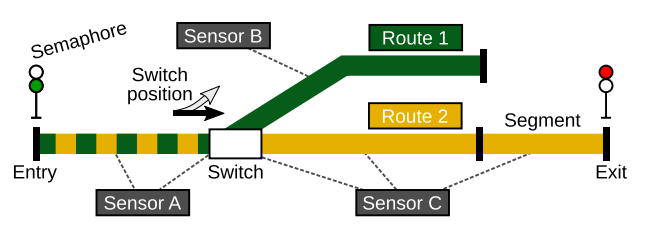
\includegraphics[width=0.7\textwidth]{figures/trainbenchmarkfig1}
	\caption{Vasúti útvonal részlet (forrás: \cite{szarnyas2018train})}
	\label{fig:trainbenchmark}
\end{figure}

 \Aref{fig:trainbenchmark}-es ábrán látható egy a trainbenchmark metamodelljére alapuló részlet. Ebben a kontextusban egy vasúti útvonal nem más mint szegmensek és váltók sorozata, illetve a belépést és a kilépést egy-egy szemafor jelzi. Ahhoz hogy biztonságos legyen a közlekedés szükség van szenzorokra, amelyek monitorozzák a különböző szegmensek és váltók kihasználtságát. Egy útvonal definiálásához ,a felsorolt elemeken kívül a váltók adott útvonalhoz tartozó pozícióját is el kell tárolnunk. Egy útvonal akkor aktív, ha a rendszerben a specifikációjának megfelelően állnak a váltók.

A metamodellezés egy tecknika arra, hogy definiájunk modellező nyelveket, ahol a metamodell specifikálja a nyelv szintaktikáját. A trainbenchmark metamodellje \aref{fig:trainbenchmarkmetamodell} -es ábrán látható.

\begin{figure}
	\centering
	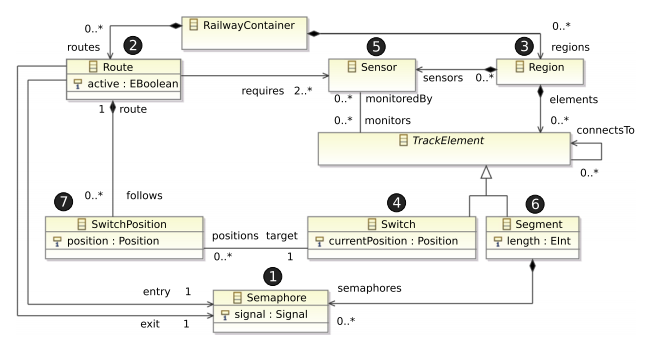
\includegraphics[width=0.7\textwidth]{figures/trainbenchmarkfig2}
	\caption{A train benchmark metamodellje. a, tartalmazási hierarchia és relációk b, öröklési relációk (forrás: \cite{szarnyas2018train})}
	\label{fig:trainbenchmarkmetamodell}
\end{figure}


\section{Gráflekérdező rendszerek}
A gráfok intuitív formalizációt nyújtanak modellezési szempontból arra, hogy úgy írhassuk le a világot ahogy az ember gondolkozik róla. Tehát mint dolgok (csomópontok) és köztük lévő kapcsolatok (élek) \cite{marton2017model}. A property gráf adatmodell kiterjeszti a gráfokat úgy, hogy címkéket/típusokat illetve tulajdonságokat ad a csúcsoknak és az éleknek. A gráf adatbázisok  alkalmasak tulajdonság gráfok tárolására, és az abban lévő adatok lekérdezésére komplex gráf minták használatával. Ilyen rendszerek például a    Neo4j \cite{neo4j}, OrientDB \cite{orientdb} és a  SparkSee \cite{sparksee}.

\begin{figure}
	\centering
	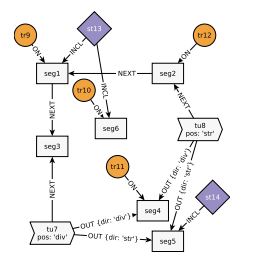
\includegraphics[width=0.7\textwidth]{figures/tulajdonsággráfpélda}
	\caption{Property gráf példa(forrás: \cite{marton2017model})}
	\label{fig:tulajdonsággráfpélda}
\end{figure}

Ahhoz hogy jobban megérthessük mi is ez az adatmodell \aref{fig:tulajdonsággráfpélda} -es ábrán látható egy példa.
\subsection{Neo4j}




\section{Modellezés és metamodellezés}
\subsection{Cypher query-k metamodellje}
\subsection{xText}
\subsection{\textsc{Viatra} jólformáltsági kényszerek}

\section{Gráfgenerálás}

ábra milyen bemenetek milyen kimenetek





